% \documentclass{beamer}
\documentclass[aspectratio=141]{beamer}
\usepackage[utf8]{inputenc}
\usepackage[T1]{fontenc}
\usepackage{mathtools}
\usepackage{graphicx}
\usepackage{caption}
\usepackage{tikz}
\usepackage{pgfplots}
\usepackage{amsmath, amssymb, amsthm}
\usepackage{mathrsfs}
\DeclareMathAlphabet{\mathdutchcal}{U}{dutchcal}{m}{n}
\SetMathAlphabet{\mathdutchcal}{bold}{U}{dutchcal}{b}{n}
\DeclareMathAlphabet{\mathdutchbcal}{U}{dutchcal}{b}{n}
\usepackage{aligned-overset}
\usepackage{color}
%\usepackage[backend=bibtex,style=numeric,sorting=nyt]{biblatex}
%\addbibresource{bibliografia.bib}
\captionsetup{labelformat=empty,labelsep=none}
%\useoutertheme{miniframes}
%\setbeamercolor{section in head/foot}{bg=blue, fg=white}
%\setbeamercolor{subsection in head/foot}{bg=blue!50, fg=white}

\newcommand{\R}{\mathbb{R}} %scorciatoia per R reali
\newcommand{\N}{\mathbb{N}} %scorciatoia per N naturali
\newcommand{\Q}{\mathbb{Q}} %scorciatioia per Q razionali
\newcommand{\V}{\mathcal{V}} %STFT
\newcommand{\F}{\mathscr{F}} %Fourier transform
\newcommand{\Fock}{\mathcal{F}} %Fock space
\newcommand{\C}{\mathbb{C}} %Complex numbers
\newcommand{\B}{\mathscr{B}} %Bounded linear operators
\newcommand{\Barg}{\mathcal{B}} %Bargmann transform
\renewcommand{\L}{\mathscr{L}} %sesquilinear form localization operator
\newcommand{\dxdo}{\,dx\,d\omega}
\newcommand{\notazione}{\underline{\textbf{Remark Notazionale}}}
\newcommand{\Log}{\ensuremath{\mathrm{Log}_-}}
\newcommand{\finire}{\fbox{\LARGE DA FINIRE}}
\newcommand{\pdfrac}[2]{\dfrac{\partial #1}{\partial #2}}
\newcommand{\pfrac}[2]{\frac{\partial #1}{\partial #2}}
\DeclareMathOperator*{\esssup}{ess\,sup}
\newcommand{\emptyline}{\phantom{ }\\}

\title[Recent results on the norm of localization operators]{Recent results on the norm of localization operators}
\date[ISPN ’80]{Laurea Magistrale in Ingegneria Matematica}
\author[F. Riccardi]{Federico Riccardi}

\usetheme{DE}

\setbeamertemplate{footline}[my footline]

\begin{document}
	


\begin{frame}
\titlepage
\end{frame}

%\setbeamertemplate{footline}{}

\begin{section}{Introduzione}
	
	\begin{frame}
		\frametitle{Introduzione}
		\textbf{Problema}: trattare un segnale, ad esempio una traccia audio, un'immagine, una misurazione di un sensore, ecc.;\\
		\pause
		\emptyline
		\textbf{Motivazioni}: analizzare il segnale ed estrarne informazioni rilevanti, filtrare componenti non desiderate, rilevare frequenze più energetiche;\\
		\pause
		\emptyline
		\textbf{Obiettivo}: localizzare il segnale in modo da concentrare il più possibile le informazioni;\\
		\pause
		\emptyline
		\textbf{Come fare}: trasformate, ad esempio la trasformata di Fourier $\F$, trasformate tempo-frequenza, come la short-time Fourier transform, operatori di localizzazione.
	\end{frame}

	\begin{frame}
		\frametitle{Introduzione}
		\framesubtitle{Principi di indeterminazione}
		L'obiettivo di localizzare un segnale si scontra con un limite fondamentale, ovvero i \emph{principi di indeterminazione}, il cui messaggio principale è:
		\begin{center}
			\emph{una funzione non può essere troppo concentrata sia in tempo che in frequenza}.
		\end{center}
		\begin{center}
			\begin{figure}
				\scalebox{1}{
				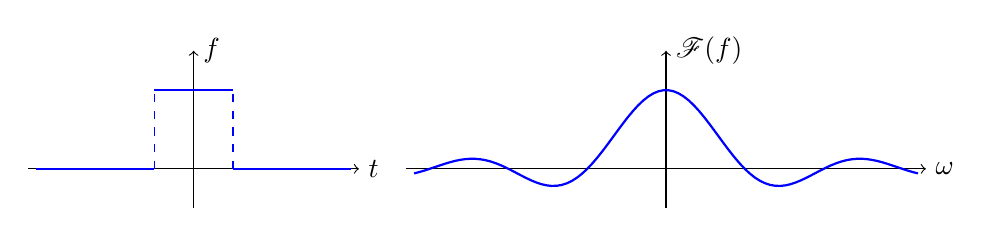
\begin{tikzpicture}
					%\draw[very thin,color=gray] (-6,-2.5) grid (6,2.5);
					\coordinate (L) at (-3,0);
					\coordinate (R) at (3,0);
					%\draw[->] (-6,0) --  (6,0);
					%\draw[->] (0, -2.5) -- (0, 2.5);
					\draw[->, shift={(L)}] (-2.1, 0) -- (2.1, 0) node[right]{$t$};
					\draw[->, shift={(L)}] (0, -0.5) -- (0, 1.5) node[right]{$f$};
					\draw[thick, blue, shift={(L)}] plot[domain=-2:-0.5] (\x,0);
					\draw[dashed, blue, shift={(L)}] (-0.5, 0) -- (-0.5, 1);
					\draw[thick, blue, shift={(L)}] plot[domain=-0.5:0.5] (\x,1);
					\draw[dashed, blue, shift={(L)}] (0.5, 0) -- (0.5, 1);
					\draw[thick, blue, shift={(L)}] plot[domain=0.5:2] (\x,0);
					
					\draw[->, shift={(R)}] (-3.3, 0) -- (3.3, 0) node[right]{$\omega$};
					\draw[->, shift={(R)}] (0, -0.5) -- (0, 1.5) node[right]{$\F(f)$};
					\draw[thick, blue, shift={(R)}] plot[domain=-3.2:3.2, samples=100] (\x, {sin(3.14*deg(\x))/(3.14*\x)});
				\end{tikzpicture}}
			\caption{Esempio di funzione ben concentrata in tempo con trasformata poco concentrata in frequenza.}
			\end{figure}
		\end{center}
	\end{frame}

	\begin{frame}
		\frametitle{Introduzione}
		\framesubtitle{Esempio: principio di indeterminazione di Heisenberg}
		\begin{theorem}
			Sia $f \in L^2(\R)$ con $\|f\|_2 = 1$ e siano $a,b \in \R$. Allora:
			\begin{equation*}
				\left(\int_{\R} (t-a)^2 |f(t)|^2 \, dt\right)^{1/2} \left(\int_{\R} (\omega-b)^2 |\F f(\omega)|^2 \, d\omega	\right)^{1/2} \geq \dfrac{1}{4 \pi}.
			\end{equation*}
			Le funzioni che raggiungono l'uguaglianza sono solo le gaussiane.
		\end{theorem}
		\pause
		\textbf{Interpretazione}: i due integrali si possono vedere come misure della concentrazione di $f$ e $\F f$ vicino ai punti $a$ e $b$, rispettivamente. Se una delle concentrazioni è ``piccola'', l'altra deve essere ``grande''.\\
	\end{frame}
	
\end{section}

\begin{section}{Short-time Fourier transform}
	\begin{frame}
		\frametitle{Short-time Fourier transform}
		La \emph{short-time Fourier transform}, in breve \emph{STFT}, è una trasformata tempo frequenza. Prima di definirla, dobbiamo introdurre gli operatori di traslazione e modulazione. Dati $x, \omega \in \R$ abbiamo:
		\begin{equation*}
			T_x f(t) = f(t-x), \quad M_{\omega} f(t) = e^{2 \pi i \omega t} f(t).
		\end{equation*}
		\pause
		La short-time Fourier transform di una funzione $f \in L^2(\R)$ rispetto alla finestra $\phi \in L^2(\R)$ è data da:
		\begin{equation*}
			\V_{\phi} f(x, \omega) = \langle f, M_{\omega} T_x \phi \rangle = \int_{\R} f(t) \overline{\phi(t-x)} e^{-2 \pi i \omega t} \, dt
		\end{equation*}
		\pause
		Per avere una buona risoluzione, bisogna scegliere una finestra ben concentrata sia in tempo che in frequenza. Per questo, ci concentriamo sulla STFT con finestra gaussiana normalizzata $\varphi(t) = 2^{1/4} e^{-\pi t^2}$.
	\end{frame}

	\begin{frame}
		\frametitle{Short-time Fourier transform}
		
	\end{frame}
\end{section}

\begin{section}{Preliminari}

	\begin{frame}
		\begin{figure}
			\centering
			\begin{tikzpicture}
				%\draw[very thin,color=gray] (-0.1,-1.1) grid (3.9,3.9);
				
				%\draw[->] (-0.2,0) -- (4.2,0) node[right] {$x$};
				\draw[->] (0,-1.2) -- (0,4.2) node[above] {$f(x)$};
				
				%\draw[color=red]    plot (\x,\x)             node[right] {$f(x) =x$};
				% \x r means to convert '\x' from degrees to _r_adians:
				%\draw[color=blue]   plot (\x,{sin(\x r)})    node[right] {$f(x) = \sin x$};
				\draw[dashed] plot[blue, domain=-2:2] (\x,{1.19*exp(-(\x)^2)}) node[right] {$f(x) = \frac{1}{20} \mathrm e^x$};
			\end{tikzpicture}
		\end{figure}
	\end{frame}

	\begin{frame}
		contenuto...
	\end{frame}
\end{section}
\begin{frame}
	contenuto...
\end{frame}

\begin{section}{Fine}
	\begin{frame}
		contenuto...
	\end{frame}

	
\end{section}

\usebeamertemplate{endpage}

\end{document}